\documentclass{beamer}
\usefonttheme[onlymath]{serif}
\usepackage[english]{babel}							%For internationalization
\usepackage[utf8]{inputenc}							%For character encoding
\usepackage{amsmath}								%For mathematical typesetting
\usepackage{amssymb}								%For mathematical typesetting
\usepackage{graphicx}								%For handling graphics
\usepackage{listings}

\newcommand{\be}{\begin{equation}}
\newcommand{\ben}[1]{\begin{equation}\label{#1}}
\newcommand{\ee}{\end{equation}}
\newcommand{\aomega}{\overset{\sim}{\omega}}				%Approximate omega

\setbeamerfont{footnote}{size=\tiny}
\beamertemplatenavigationsymbolsempty
\setbeamerfont{page number in head/foot}{size=\large}
\setbeamertemplate{footline}[frame number]
\lstset{breaklines=true,basicstyle=\tiny}

\title
{A High-Order Conservative Eulerian Simulation Method for Vortex Dominated Flows}
\subtitle{AIAA Aviation 2016}
\author[Bevan] % (optional, for multiple authors)
{J.~Bevan}
\institute[UMass Lowell] % (optional)
{
 Prof. D.J. Willis, Associate Professor\\
\vspace{0.5 cm}
  Department of Mechanical Engineering\\
  University of Massachusetts at Lowell\\
\vspace{0.5 cm}
 June 13, 2016
}
\date[June 2016] % (optional)
{}
\subject{Discontinuous Galerkin}

\begin{document}
\frame[plain,noframenumbering]{\titlepage}
%NEW SECTION
\section{Abstract}
\frame[shrink]{\frametitle{\textbf{\secname}: \subsecname}
A high-order, conservative Eulerian method is presented for the simulation of vortex dominated inviscid fluid flows. The primitive variable incompressible Euler equations are recast in the velocity-vorticity form to explicitly enforce conservation of vorticity. The advection of the vorticity is then calculated via a two-step process: the velocity field is determined by evaluation of the Biot-Savart integral, and then a line-based discontinuous Galerkin (DG) Eulerian spatial discretization scheme is applied to accurately advect the vorticity field. The accuracy and convergence of this method was examined for test cases where an analytical solution exists, as well as more challenging test cases which lack an analytical solution. The convergence rate behavior is chiefly controlled by the error in the calculated velocity field. Velocity errors are due to two factors: the approximation of the Biot-Savart integral with a desingularized form, and reduced quadrature convergence for the nearly singular integral. Solver parameters were chosen to balance these two effects resulting in nearly optimal convergence of the overall method in the analytical test, and high-order convergence in the qualitative test case.
}

\section{Introduction}
\subsection{Presentation Structure} 
\frame{\frametitle{\textbf{\secname}: \subsecname}
\begin{itemize}
\item Introduction
\item Theory
\item Methodology
\item Implementation
\item Results
\item Discussion
\item Conclusion
\end{itemize} 
}

\subsection{Goals of Technique} 
\frame{\frametitle{\subsecname}
Goals:
\begin{itemize}
\item  Development of a high-order solver for inviscid incompressible vorticity-dominated flows in 2D
	\begin{itemize}
	\item High-order advective solver capable of mixed order flux handling
	\item High-order Biot-Savart evaluation routine
	\end{itemize}
\end{itemize}
Contributions:
\begin{itemize}
\item Complete high-order method for velocity-vorticity inviscid flow
\item Validation of solver and underlying Eulerian vortex approach
\item Evaluation of convergence, error, and performance of method and solver
\end{itemize} 
}

\subsection{Motivation} 
\frame{\frametitle{\subsecname}
\begin{itemize}
\item Direct solution of Navier-Stokes impractical for many fluid problems
\item Vorticity-velocity formulation well-suited for inviscid, incompressible, vortex dominated flows
\item Lagrangian vortex methods are common approach\footnotemark$^,$\footnotemark, but face several challenges\footnotemark
\item Initial vortex points become disorganized, re-meshing etc. required
\item Eulerian approach avoids disorganization, extendable to high order
\item Brown et al. successful with Eulerian approach for low order FVM\footnotemark \,suggests high-order extension possible
\end{itemize}
\footnotetext[1]{J. Strain. Fast adaptive 2D vortex methods. Journal of computational physics 132.1 (1997): 108-122.}
\footnotetext[2]{Moussa, C., Carley, M. J. (2008). A Lagrangian vortex method for unbounded flows. International journal for numerical methods in fluids, 58(2), 161-181.}
\footnotetext[3]{J. Strain. 2D vortex methods and singular quadrature rules. Journal of Computational Physics 124.1 (1996): 131-145.}
\footnotetext[4]{R.E. Brown. Rotor Wake Modeling for Flight Dynamic Simulation of Helicopters. AIAA Journal, 2000. Vol. 38(No. 1): p. 57-63.}
}

\subsection{Proposed Method} 
\frame{\frametitle{\subsecname}
\begin{itemize}
\item Eulerian representation of velocity and vorticity
\item Solution of inviscid velocity-vorticity PDE
\item Velocity evaluation via eval of Biot-Savart kernel\footnotemark
\item Vorticity advection via a line-DG\footnotemark \,approach
\item Method of lines, explicit time-stepping with Runge-Kutta\footnotemark
\end{itemize} 
\footnotetext[5]{Winckelmans, G. S., and A. Leonard. Contributions to vortex particle methods for the computation of three-dimensional incompressible unsteady flows. Journal of Computational Physics 109.2 (1993): 247-273.}
\footnotetext[6]{P.O. Persson. A Sparse and High-Order Accurate Line-Based Discontinuous Galerkin Method for Unstructured Meshes. J. Comp. Phys., Vol. 233, pp. 414-429, Jan 2013.}
\footnotetext[7]{Niegemann, Jens, Richard Diehl, and Kurt Busch. Efficient low-storage Runge–Kutta schemes with optimized stability regions. Journal of Computational Physics 231.2 (2012): 364-372.}
}

\section{Theory}
\subsection{Navier-Stokes: Velocity-vorticity form} 
\frame{\frametitle{\textbf{\secname}: \subsecname}
Navier-Stokes momentum equation
 \be \rho \left(\frac{\partial \mathbf{u}}{\partial t} + \mathbf{u} \cdot \nabla \mathbf{u} \right) = -\nabla p + \mu \nabla^2 \mathbf u + \tfrac13 \, \mu \nabla (\nabla\cdot\mathbf{u}) \ee
where $u$ is the velocity field, $p$ is the pressure field, and $\rho$ is the density.  Define \textit{vorticity} as
\be \mathbf{\omega} = \nabla \times \mathbf{u} \ee
Navier-Stokes can be recast as
\ben{VV3D} \frac{\partial \omega}{\partial t} +  \mathbf{u} \cdot \nabla \omega - \omega \cdot \nabla  \mathbf{u} = S(x,t)\ee
 viscous generation of vorticity, $S$
}

\subsection{Velocity-vorticity form} 
\frame{\frametitle{\subsecname}
Advantages:
\begin{itemize}
\item Explicit conservation of vorticity.
\item Frequently distribution of the vorticity is sparse.
\item No pressure term.
\end{itemize}
Simplified in 2D, vortex stretching zero. Express in terms of vortex flux $f_i(\omega)=u_i\,\omega$
\ben{VV2DB} \frac{\partial \omega}{\partial t} + \frac{\partial f}{\partial x_i}= S(x,t)\ee
}

\subsection{Velocity Evaluation} 
\frame{\frametitle{\subsecname}
For incompressible flows velocity related to vorticity by
\be \nabla^2 u = -\nabla \times \omega \ee
Invert to obtain Biot-Savart integral
\ben{BS} u(x^*) = \int_\Omega K(x^*,x) \times \omega(x) dx \ee
$x^*$ is velocity eval point, $x$ is non-zero vorticity domain, $K(x^*,x)$ singular Biot-Savart kernel\footnotemark
\ben{BSkern} K(x^*,x) = \frac{-1}{2 \pi} \frac{x^*-x}{|x^*-x|^2} \ee

\footnotetext[8]{Beale, J. Thomas, and Andrew Majda. High order accurate vortex methods with explicit velocity kernels. Journal of Computational Physics 58.2 (1985): 188-208.}
}

\subsection{Kernel De-singularization: Two Viewpoints} 
\frame{\frametitle{\subsecname}
\begin{itemize}
\item Lagrangian: Singularity in Biot-Savart kernel generates non-physical velocities near vortex points, de-singularize by approximation of Dirac delta function using finite cutoff radius $\delta$.
\item Lagrangian: Heuristically, one deals with vortex ``blobs''.
\item Eulerian: Vorticity is not confined to points, but spatially varying; what purpose does de-singularization serve? Strictly practical.
\item Eulerian: While Biot-Savart kernel converges analytically, no guarantees numerically. Quadrature assumes polynomial basis appropriate approximation.
\item Eulerian: De-singularization means to an end, improve quadrature convergence qualities.
\end{itemize}
}

\subsection{Convergence of Biot-Savart Integral} 
\frame{\frametitle{\subsecname}
\begin{itemize}
\item Nearly singular nature of Biot-Savart kernel difficult to integrate numerically
\item Smaller the cutoff radius, larger quadrature errors
\item Larger cutoff radius, larger velocity approximation errors
\item Cutoff radius should be selected to balance both
\end{itemize}
\begin{figure}
\centering
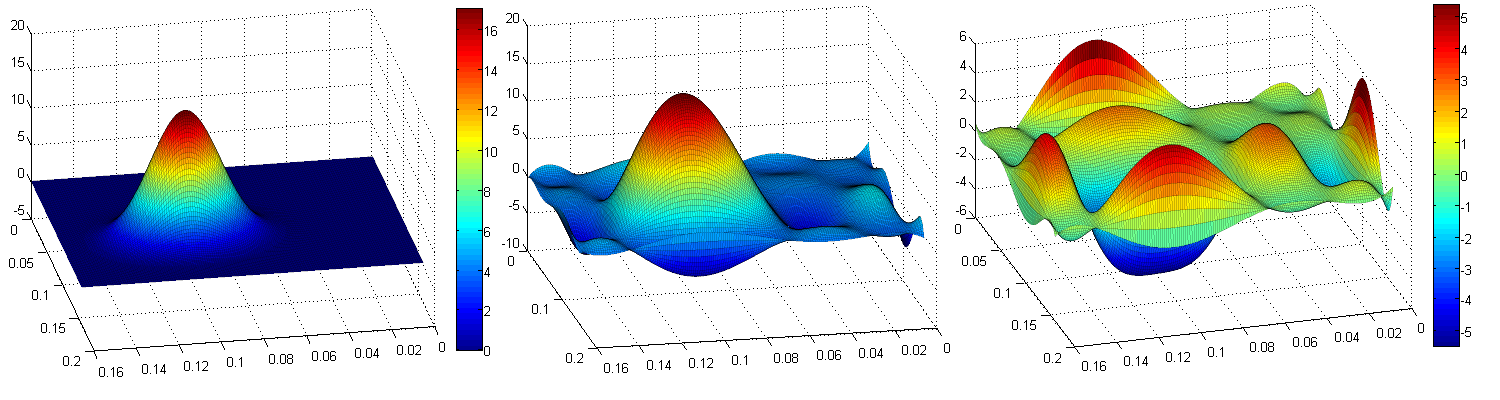
\includegraphics[width=4.5in]{wKcomp.PNG}
\end{figure}
}

\subsection{Discontinuous Galerkin (DG)} 
\frame{\frametitle{\subsecname}
- Why DG vs others?\\
We seek to solve the PDE Eqn.\,\eqref{VV2DB}. An approximate solution $\aomega$ has residual
\ben{VV2D} \frac{\partial \aomega}{\partial t} + \frac{\partial f}{\partial x_i} = R(x)\ee
1-D case, vorticity sources omitted for simplicity.\\
DG approach\footnotemark: minimize the $L^2$ norm by orthogonal projection of residual onto approximating space. Complete basis made from test functions $\phi_j$, so:
\be \int_\Omega R(x) \phi_j \;dx = 0 \quad\mbox{for all}\; j\ee
Substituting residual with conservation PDE yields:
\ben{yams} \int_\Omega \frac{\partial \aomega}{\partial t} \, \phi_j \;dx + \int_\Omega \frac{\partial f(\aomega)}{\partial x} \, \phi_j \;dx = 0 \quad\mbox{for all}\; j\ee

\footnotetext[9]{W.H Reed and T.R. Hill. Triangular mesh methods for the neutron transport equation. 1973.}
}

\frame{\frametitle{\subsecname (cont.)}
Use same space for both test functions and and approximation, so Mth order vorticity approximation is
\be \omega(x,t) \approx \aomega(x,t) = \sum_{i=0}^M a_i(t)\psi_i(x)\ee
Substitute into Eqn.\,\eqref{yams} and integrate by parts second term:
\ben{DGtemp} \sum_{i=0}^M \left[ \frac{d a_i(t)}{dt}\int_{x_L}^{x_R}\psi_i(x)  \, \phi_j(x) \;dx \right]
+ f\phi_j(x) \Big|^{x_R}_{x_L} 
- \int_{x_L}^{x_R} f(\aomega) \, \frac{d \phi_j(x)}{d x} \;dx = 0 \ee
Note: Local solution to PDE on an element.

}

\frame{\frametitle{\subsecname (cont.)}
All local solutions decoupled, also vorticity multiply defined at overlapping element boundaries. Recover global solution and treat element boundaries via an upwind flux function\footnotemark (similar to finite volume method)
\be \hat{f}_{upwind}(x^+,x^-)=u\{\!\{\aomega\}\!\} + \frac{|u|}{2}[[\aomega]]\ee
where $\{\!\{\omega^+\}\!\} = \frac{\omega^++\omega^-}{2}$ and $[[\omega]]=\omega^+-\omega^-$\\
\vspace{0.2cm}
Applying change of variables to map to arbitrary computational element $X\in[-1,1]$ results in:
\ben{DGtemp2} \frac{\Delta x}{2}	\sum_{i=0}^M \left[ \frac{d a_i}{dt}	\int_{-1}^{1}\psi_i  \, \phi_j \;dX \right]
+\hat{f}\phi_j \Big|^{x_R}_{x_L} 
- \int_{-1}^{1} f(\aomega) \, \frac{d \phi_j}{dX} \;dX = 0 \ee

\footnotetext[10]{Hesthaven, Jan S., and Tim Warburton. Nodal discontinuous Galerkin methods: algorithms, analysis, and applications. Vol. 54. Springer Science \& Business Media, 2007.}
}

\subsection{Solver Overview}
\begin{frame}[fragile]\frametitle{\subsecname}
\begin{lstlisting}[language=Matlab]
Define problem parameters
Define solver parameters
Calculate derived solver parameters
Setup intitial conditions
Initialize solver
%Time stepping
for t=0 to end
   if datalog?=yes
      save system state to file and plot
   end
   %Loop through RK stages
   for s=1 to last_stage
      %For elements above threshold
      for each vorticity source
         calculate velocity contributions
      end
      %Calculate semi-discrete system terms
      interpolate boundary_vorticity
      calculate numerical_fluxes
      calculate total_surface_flux
      calculate internal_stiffness_flux
		
      vorticity_rate_of_change=...
         internal_stiffness_flux - total_surface_flux
		
      RK_stage= (RK_coeff_a*RK_stage) +...
         (time_step * vorticity_rate_of_change)
      vorticity= vorticity + RK_coeff_b * RK_stage
   end
end
\end{lstlisting}
\end{frame}

\section{Methodology}
\subsection{Method Specific Choices} 
\frame[shrink]{\frametitle{\textbf{\secname}: \subsecname}
\begin{itemize}
\item Choose basis functions to be the interpolating Lagrange polynomials
\be \psi_i(x) =\ell_i(x) = \prod_{\substack{p=0\\ p\neq i}}^M \frac{x-x_p}{x_i-x_p}\ee
\item Choose vorticity interpolation nodes to be the Gauss-Legendre points, collocate with quadrature points, results in simplification of mass matrix
\ben{diag} \int \ell_i(x) \ell_j(x) dx = \delta_{ij} w_j \ee
\item Take line-DG\footnotemark[6] approach, form 2D basis as tensor product of 1D bases
\be f(x,y) \approx \left[\sum_{j=0}^L z_j \ell_j(y) \right] \times \left[ \sum_{i=0}^M z_i \ell_i(x) \right] = \sum_{j=0}^M \sum_{i=0}^M z_{ij} \ell_j \ell_i =  \sum_{j=0}^M z_{ij} \ell_j \sum_{i=0}^M  \ell_i \ee
\end{itemize}
}

\frame{\frametitle{\subsecname (cont.)}
\begin{itemize}
\item The PDE is now solved along each tensor direction
\ben{DGJoshTemp} \frac{\Delta x}{2}	\sum_{i=0}^M \left[ \frac{d z_{ij}}{dt}	\int_{-1}^{1}\ell_i  \, \ell_j \;dX \right]
+\hat{f}\ell_j \Big|^{x_R}_{x_L} 
- \int_{-1}^{1} f(\aomega) \, \ell_j' \;dX = 0 \ee
\item The rate of change at each node is the sum of the contribution along each tensor direction
\be \frac{\partial \omega_{ij}}{\partial t} = (\frac{\partial \omega_{ij}}{\partial t})_{x-line} + (\frac{\partial \omega_{ij}}{\partial t})_{y-line} \ee
\end{itemize}
\begin{figure}
\centering
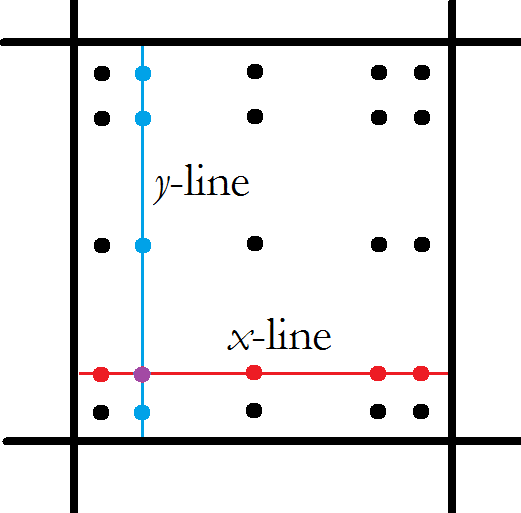
\includegraphics[width=1.5in]{lineDGelemDiag.PNG}
\end{figure}
}

\subsection{Flux Interpolation and Modified Quadrature} 
\frame{\frametitle{\subsecname}
\begin{itemize}
\item Interpolate flux via product of interpolations of vorticity and velocity (rather than interpolation of their product)
\be \begin{split}\int u(x) \omega(x) \ell_j'(x) \;dx &\approx \int \sum_i^M u_i \ell_i(x) \sum_k^M \omega_k \ell_k(x) \;\ell_j'(x) \;dx\\
&=\sum_i^M u_i \sum_k^M \omega_k \int \ell_i(x) \ell_k(x) \ell_j'(x) \;dx
\end{split}\ee
\item To do so, generate a matrix of modified quadrature weights
\be \int \ell_i(x) \ell_k(x) \ell_j'(x) \;dx = \mathbf{W}_{ikj} \ee
\item The resultant quadrature rule is now
\ben{modQuad} \int u(x) \omega(x) \ell_j'(x) \;dx \approx \mathbf{u}_i^T \mathbf{W}_{ikj} \, \boldsymbol{\omega}_k \ee
for each $j$th weighting basis function.
\end{itemize}
}

\subsection{Modified Quadrature Advantages} 
\frame{\frametitle{\subsecname}
\begin{itemize}
\item Able to extract \textit{more} information out of \textit{same} number of interpolation points with superior convergence of stiffness integral compared to standard Gauss-Legendre rule (integrate N point vorticity/velocity- 2N+2 order interpolation vs. N+1 order interpolation exactly)
\item Including derivative of the weighting basis in integral for quadrature weight matrix means integrated exactly \textit{a priori}
\item Order and definition of the Lagrange basis functions for vorticity and velocity interpolations are \textit{decoupled}
\item Able to use Gauss-Legendre points for vorticity and Lobatto for velocity (avoids extra boundary velocity calcs)
\end{itemize}
}

\section{Implementation}
\subsection{Structured Tensor Mesh} 
\frame{\frametitle{\textbf{\secname}: \subsecname}
\begin{itemize}
\item Vorticity and velocity stored ``line-wise'' along tensor directions per element.
\item Advection and velocity calcs operate line-wise
\end{itemize}
\begin{figure}
\centering
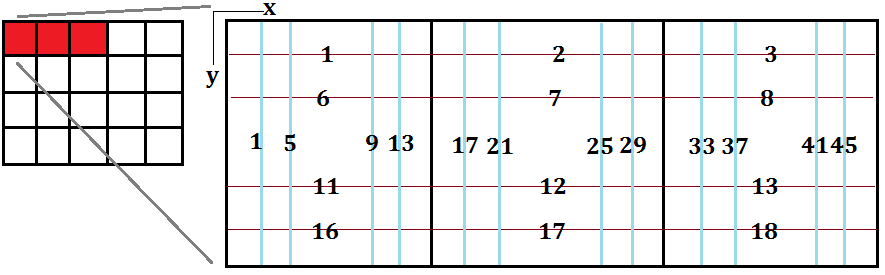
\includegraphics[width=4in]{streams.PNG}
\end{figure}
}

\subsection{Mass Matrix} 
\frame{\frametitle{\subsecname}
Making use of  Eqn.\,\eqref{diag} the mass matrix
\be \boldsymbol{M} = \frac{\Delta x}{2} \sum_{i=0}^M \left[ \frac{d z_{ij}}{dt}	\int_{-1}^{1}\ell_i  \, \ell_j \;dX \right] \ee
is diagonalizable. We can simplify Eqn.\,\eqref{DGJoshTemp}:
\ben{DGJoshTemp2} \frac{d \aomega_j}{dt} \frac{w_j \Delta x}{2}
+\hat{f}\ell_j \Big|^{x_R}_{x_L} 
- \int_{-1}^{1} f(\aomega) \, \ell_j' \;dX = 0 \ee
}

\subsection{Stiffness Matrix} 
\frame{\frametitle{\subsecname}
\begin{itemize}
\item Velocity nodes for a particular line don't coincide with vorticity nodes, but are still co-linear
\item Only the velocity component directed along the line is needed at a particular velocity node
\end{itemize}
\begin{figure}
\centering
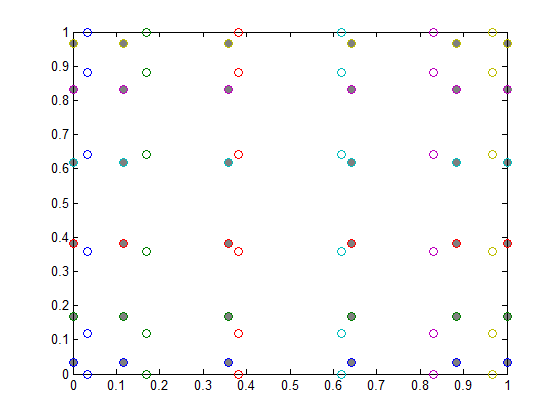
\includegraphics[width=3in]{VelocityLobatto.PNG}
\end{figure}
}

\frame{\frametitle{\subsecname (cont.)}
\begin{itemize}
\item Apply modified quadrature rule to the stiffness term
\be \boldsymbol{K} = \int_{-1}^{1} f(\aomega) \, \ell_j' \;dX \ee
yields:
\ben{DGJoshTemp3} \frac{d \aomega_j}{dt} \frac{w_j \Delta x}{2}
+\hat{f}\ell_j \Big|^{x_R}_{x_L} 
- \mathbf{u}^T \mathbf{W}_{--j} \, \boldsymbol{\omega} = 0 \ee
\item Rearrange to obtain ODE in time:
\ben{DGJosh} \frac{d \aomega_j}{dt}
=\frac{2}{w_j \Delta x} \left[\mathbf{u}^T \mathbf{W}_{--j} \, \boldsymbol{\omega} - \hat{f}\ell_j \Big|^{x_R}_{x_L}\right]  \ee
\end{itemize}
}

\subsection{Velocity Evaluation} 
\frame{\frametitle{\subsecname}
\begin{itemize}
\item Calculate velocity at all velocity nodes by summation of contribution from all vorticity using de-singularized kernel and Gauss-Legendre quadrature
\be u(x^*)= \sum_{E=1}^{N_{mask}} [\omega_{pre}]^TK_{\delta}(x^*-[x_E]) \ee
\be \omega_{pre} = [\omega(x_E)].*[w_i \otimes w_j]\ee
\item Pre-multiplication of particular elemental vorticity source by outer product of Gauss-Legendre quadrature weights and computing as vector-vector product saves great deal of computational effort (2000\% in current code)
\item Kernel values pre-calculated for ``generalized'' reference frame
\end{itemize}
}

\subsection{Kernel value calculations} 
\frame{\frametitle{\subsecname}
\begin{itemize}
\item Constant re-calculation of kernel values computationally expensive, but storing all values at start not possible due to memory needs scaling as $Np^4K^4$
\item Solution: calculate for generalized reference frame and map as needed for each vorticity element source
\end{itemize}
\begin{figure}
\centering
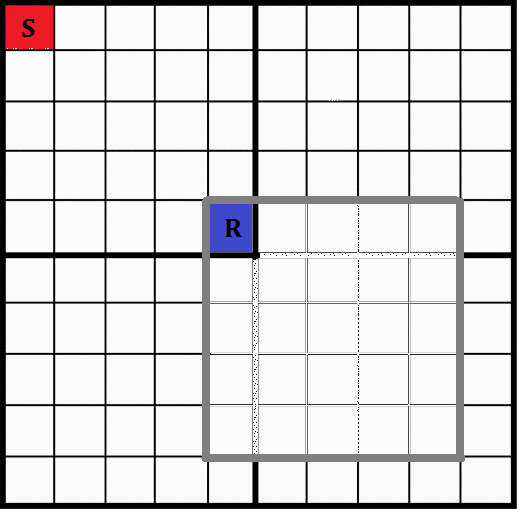
\includegraphics[width=2in]{GlobalKernel.PNG}
\end{figure}
}

\subsection{Explicit Time-Stepping} 
\begin{frame}[fragile]\frametitle{\subsecname}
\begin{itemize}
\item Method of lines approach to semi-discrete system
\item Low-storage explicit Runge-Kutta method used
\item 14 stage-4th order ``NRK14C'' used to maximize stable time-step\footnotemark[7]
\item Stability region almost 1.9 times larger per stage along negative real axis, chief consideration for dissipative upwind DG schemes
\end{itemize}
\begin{lstlisting}
for t=0:delt:EndTime %Step
    for i=1:nS %Stage
        (Velocity calculations)
        (semi-discrete calculations for advection)
        wx_dt= permute(Stiff_x-SurfFlux_x,[4 1 3 2]);
        wy_dt= reshape(reshape(...
	Stiff_y-SurfFlux_y,K(2),[])',Np,1,[]);
        
        k2= RKa(i)*k2 + delt*(wx_dt+wy_dt);
        wx= wx+RKb(i)*k2;
        wy= reshape(reshape(wx,K(1)*Np,[])',Np,1,[]);
    end
end
\end{lstlisting}
\end{frame}

\section{Results}
\subsection{Validating Test Cases} 
\frame{\frametitle{\textbf{\secname}: \subsecname}
\begin{itemize}
\item Perlman: Stationary vortex\footnotemark
\ben{PerlW} \omega(z)=(1-|z|^2)^7, \; |z|\leq 1  \quad \omega(z)=0, \;|z|>1 \quad z^2=x^2+y^2 \ee
\item Has analytical solution to vorticity and velocity fields
\ben{PerlU} u(z,t)=f(|z|)\binom{y}{-x} \ee
where
\[
f(|z|)=
\begin{cases}
    -\frac{1}{16|z|^2}(1-(1-|z|^2)^8)	& |z| \leq 1\\
    -\frac{1}{16|z|^2} 			& |z|>1
\end{cases}
\]
\end{itemize}
\footnotetext[11]{M. Perlman. On the accuracy of vortex methods, J. Comput. Phys. 59 (1985) 200–223.}
}

\subsection{Comparison of Cutoff Radius Effects(P)}
\frame{\frametitle{\subsecname}
\begin{figure}
\centering
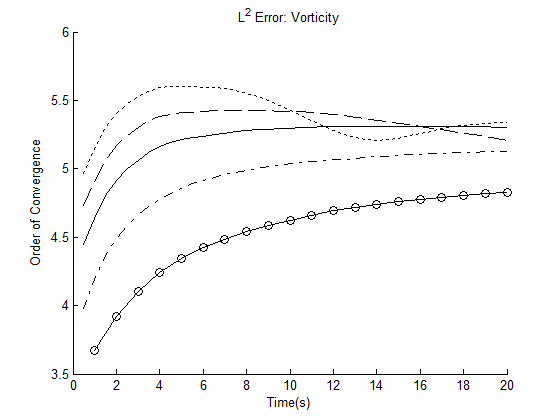
\includegraphics[width=0.8\textwidth]{CutoffW.PNG}
\caption{\label{fig:CutoffW}Comparison of convergence effects on vorticity by cutoff radius for $\delta/\Delta x$=0.1(..), 0.2(- -), 0.3(-), 0.5(-.), 0.9(-o).}
\end{figure}
}

\frame{\frametitle{\subsecname (cont.)}
\begin{figure}
\centering
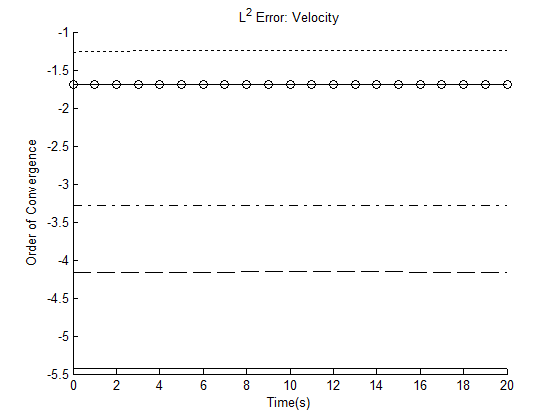
\includegraphics[width=0.8\textwidth]{CutoffU.PNG}
\caption{\label{fig:CutoffU}Comparison of convergence effects on velocity by cutoff radius for $\delta/\Delta x$=0.1(..), 0.2(- -), 0.3(-), 0.5(-.), 0.9(-o).}
\end{figure}
}

\subsection{Observed Convergence Rate of Various Orders(P)}
\frame{\frametitle{\subsecname}
\begin{figure}
\centering
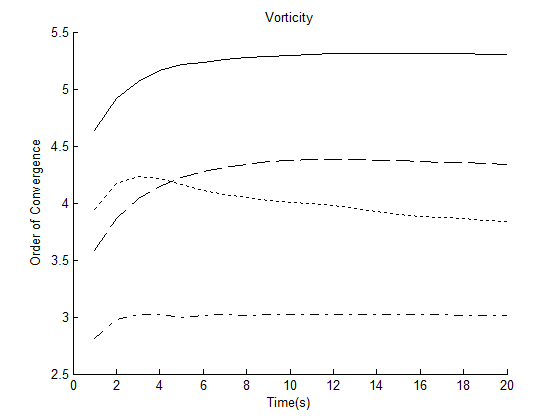
\includegraphics[width=0.8\textwidth]{Porder.PNG}
\caption{\label{fig:Porder}Comparison of convergence rate for various order methods: 3rd(-.), 4th(..), 5th(- -), and 6th(-).}
\end{figure}
}

\frame{\frametitle{Validating Test Cases}
\begin{itemize}
\item Strain: Interacting vortex patches\footnotemark
\ben{StrainV} \omega(x,y,0) = \sum_{j=1}^m \Omega_j exp(-((x-x_j)^2 + (y-y_j)^2)/\rho_j^2) \ee
\begin{table}
\centering
\caption{Interacting Vortex Patch Parameters}\label{table:StrainTable}
\begin{tabular}{lllll}
\hline
j & $x_j$    & $y_j$    & $\rho_j$ & $\Omega_j$ \\ \hline
1 & -0.6988 & -1.7756 & 0.6768  & -0.4515   \\
2 & 1.4363  & -1.4566 & 0.3294  & 0.4968    \\
3 & -0.1722 & 0.4175  & 0.5807  & -0.9643   \\
4 & -1.5009 & -0.0937 & 0.2504  &  0.3418    \\ \hline
\end{tabular}
\end{table}
\end{itemize}
\footnotetext[12]{J. Strain. 2D vortex methods and singular quadrature rules. Journal of Computational Physics 124.1 (1996): 131-145.}
}

\subsection{Approximated Convergence Rate(S)}
\frame{\frametitle{\subsecname}
\begin{figure}
\centering
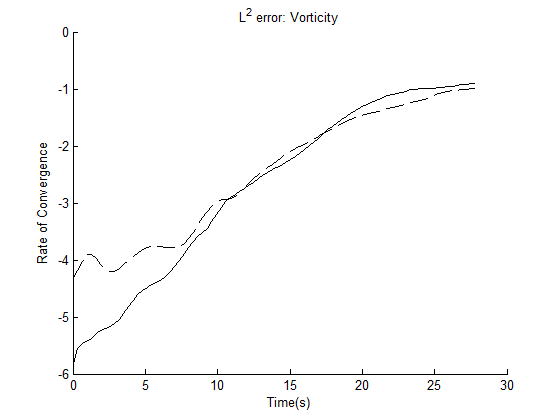
\includegraphics[width=0.8\textwidth]{Strain4vs6.PNG}
\caption{\label{fig:Strain4vs6}Dependency of rate of convergence on order of method, for a 4th order(- -) and 6th order(-) method. }
\end{figure}
}

\frame{\frametitle{\subsecname (cont.)}
\begin{figure}
\centering
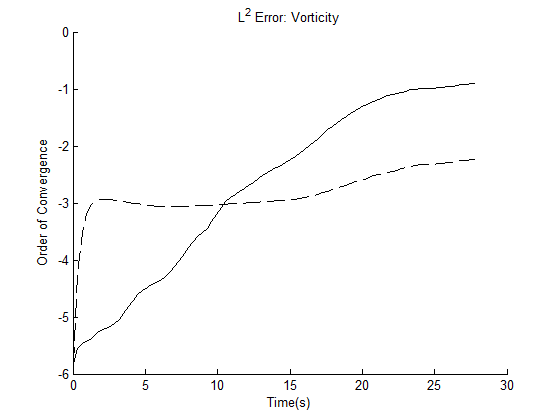
\includegraphics[width=0.8\textwidth]{Strain6vs6.PNG}
\caption{\label{fig:Strain6vs6}Dependency of rate of convergence on cutoff radius in sixth order method, for a $\delta/\Delta x$= 0.5(- -) and 0.25(-). }
\end{figure}
}

\frame{\frametitle{Qualitative Comparison w/ Previous Work$^{12}$}
\begin{figure}
\centering
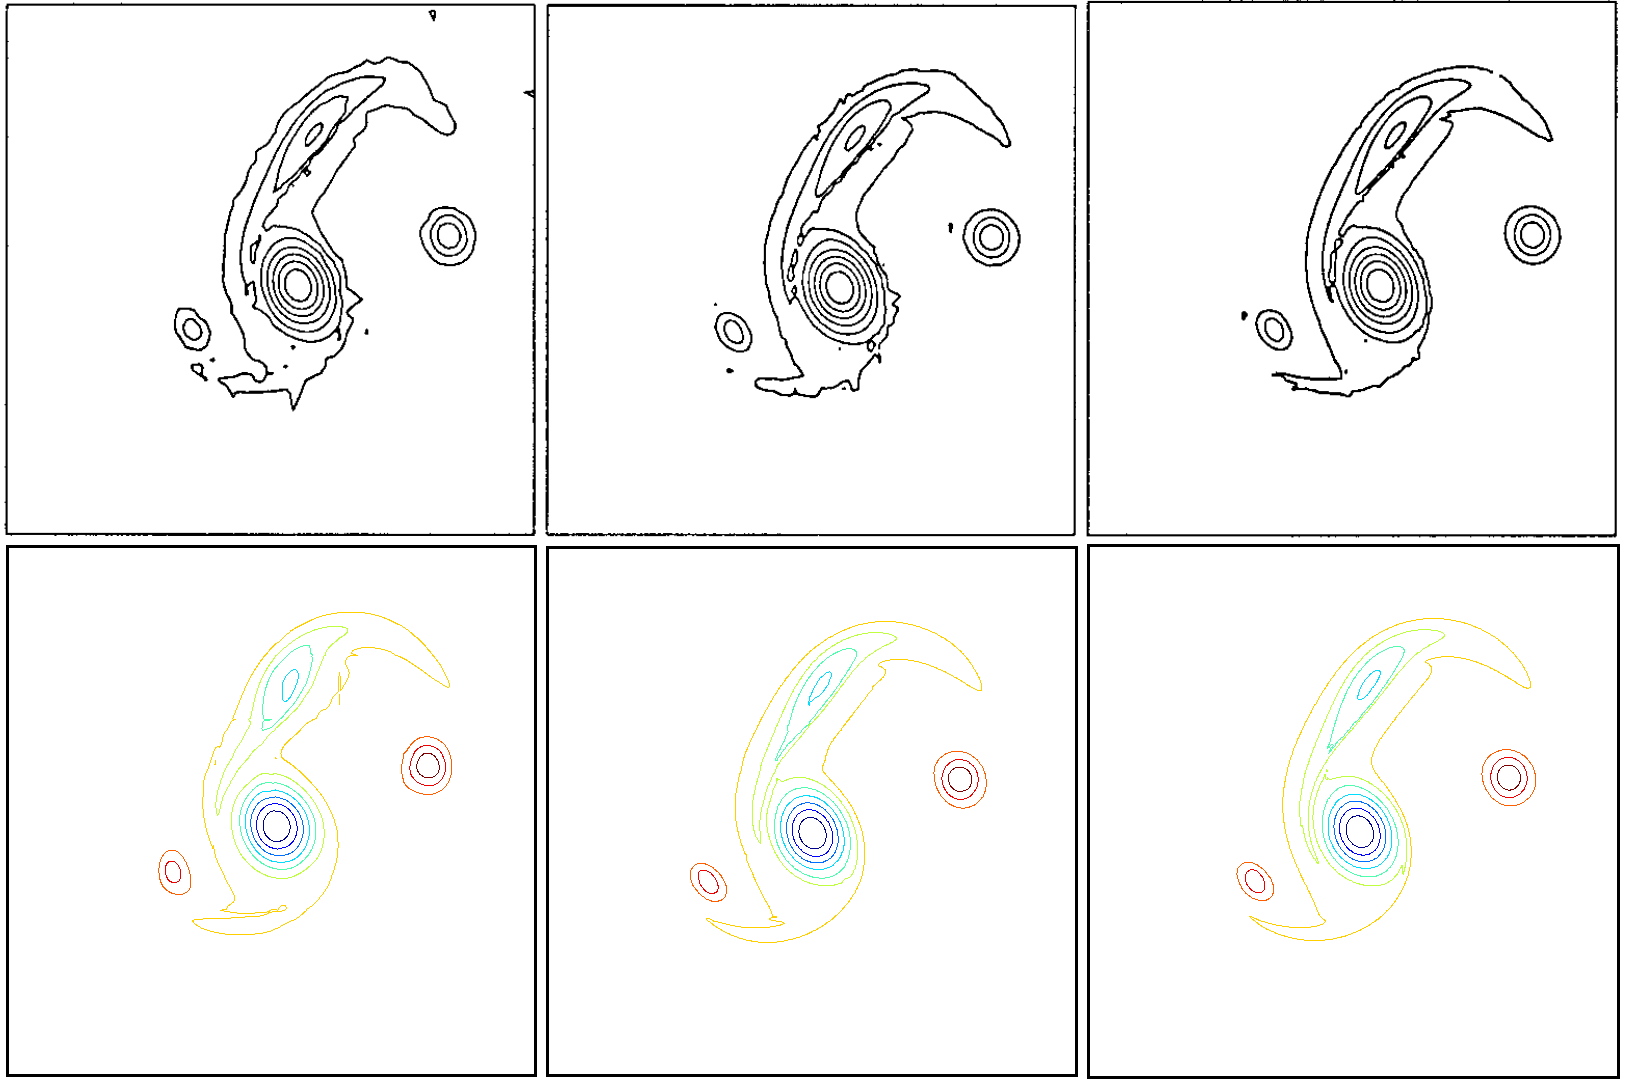
\includegraphics[width=0.9\textwidth]{StrainCompR.PNG}
\caption{\label{fig:StrainComp}Comparison of Strain's results with present method t=28. Left to right, top to bottom, DOF= 6400, 12800, 25600; 3136, 7056, 63504. Reprinted with permission from Elsevier. }
\end{figure}
}


\frame{\frametitle{Validating Test Cases}
\begin{itemize}
\item Koumoutsakos: Elliptical vortex\footnotemark
\ben{KoumEqn} \omega^{II}(x,y,0)_{mod} = 20(1-((x/a)^2+(y/b)^2)^2/0.8^4 ) \quad a=1, \; b=2 \ee
\end{itemize}
\footnotetext[13]{P. Koumoutsakos. Inviscid axisymmetrization of an elliptical vortex, J. Comput. Phys. 138 (1997) 821–857.}
\subsection{Qualitative Comparison of Vorticity(S)}
}

\subsection{Qualitative Comparison of Vorticity(K)}
\frame{\frametitle{\subsecname}
\begin{figure}
\centering
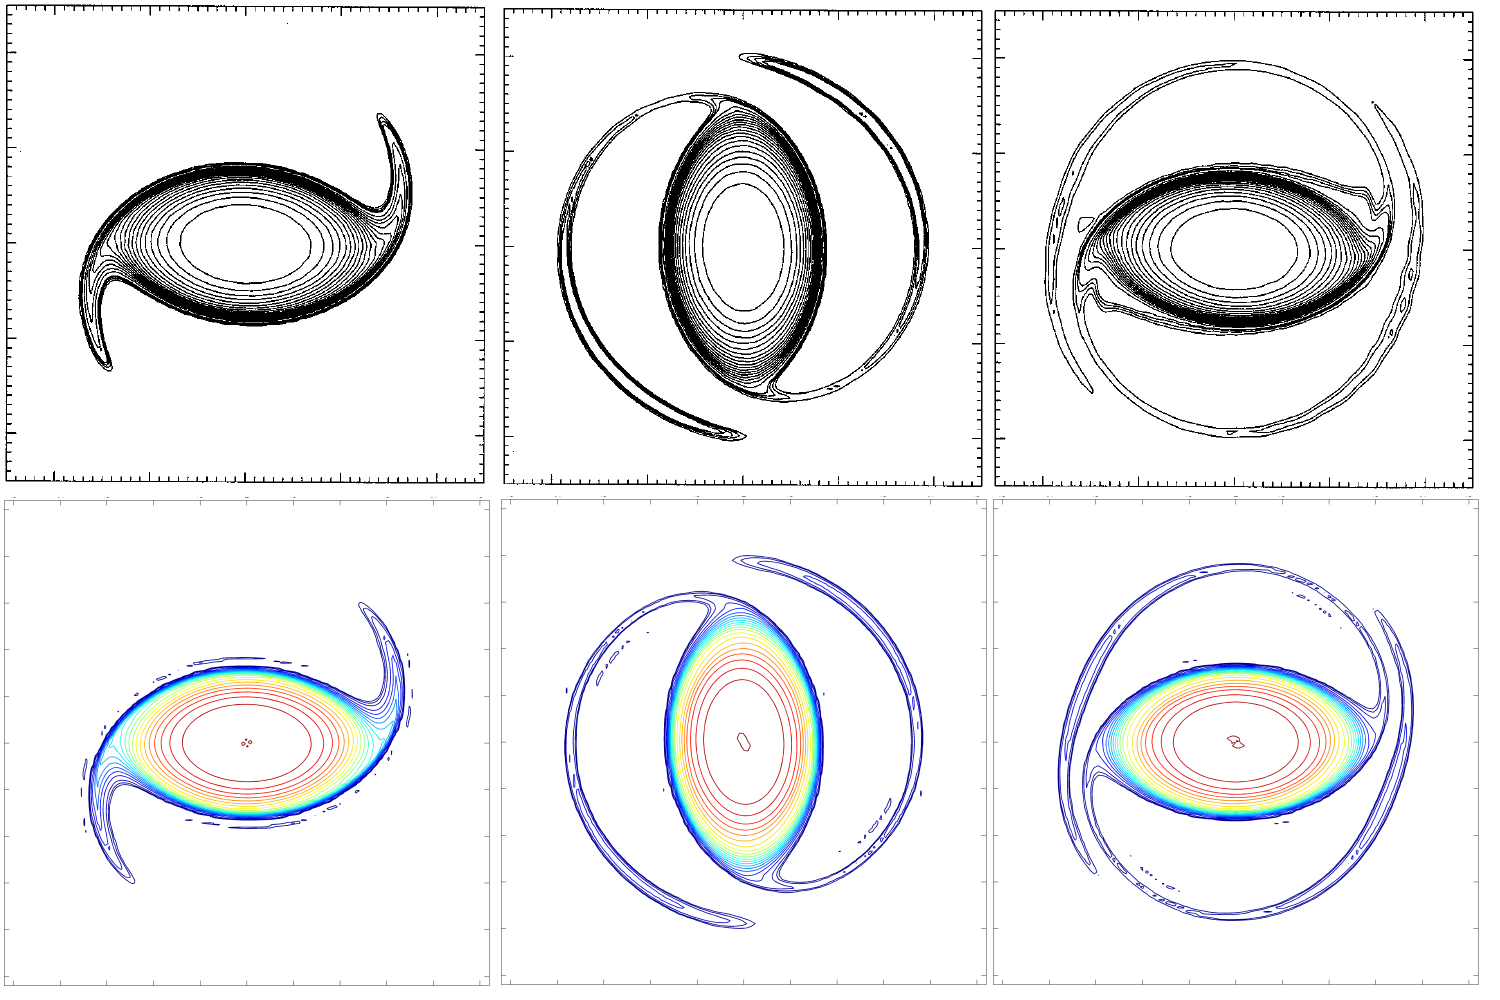
\includegraphics[width=0.9\textwidth]{KoumComp1R.PNG}
\caption{\label{fig:KoumComp1}Comparison of vorticity, Koumoutsakos (top) and present method (bottom). From left to right, top to bottom t=1, 2, 4; 0.80, 1.93, 2.32. Reprinted with permission from Elsevier.}
\end{figure}
}

\frame{\frametitle{\subsecname (cont.)}
\begin{figure}
\centering
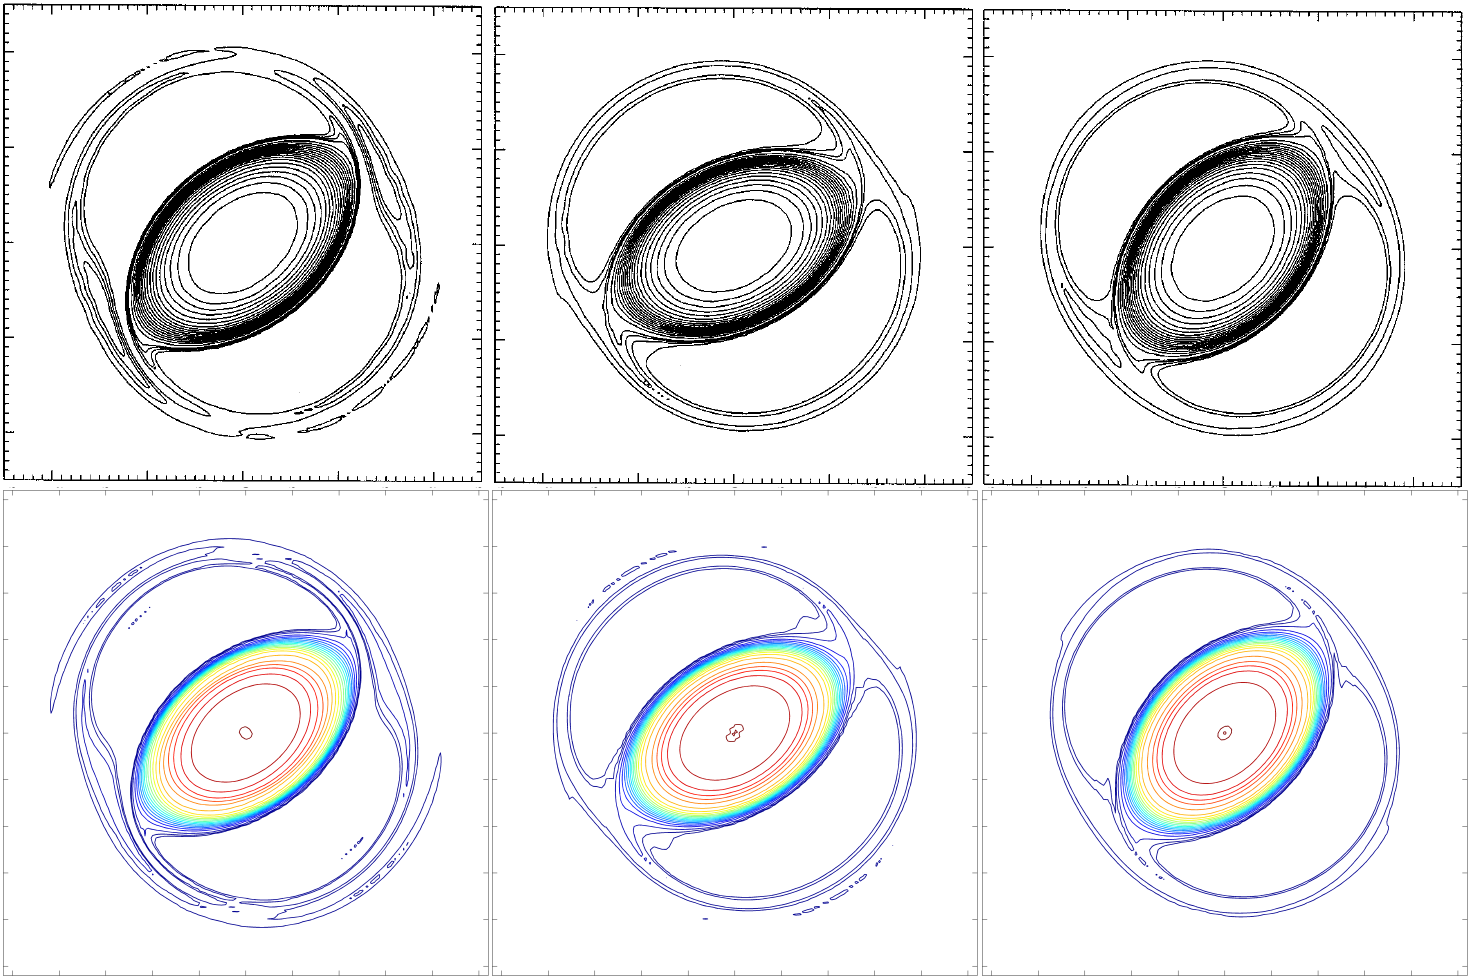
\includegraphics[width=0.9\textwidth]{KoumComp2R.PNG}
\caption{\label{fig:KoumComp2}Comparison of vorticity, Koumoutsakos (top) and present method (bottom). From left to right top to bottom,: t=6, 12, 18; 5.94, 11.99, 17.94. Reprinted with permission from Elsevier.}
\end{figure}
}

\frame{\frametitle{\subsecname (cont.)}
\begin{figure}
\centering
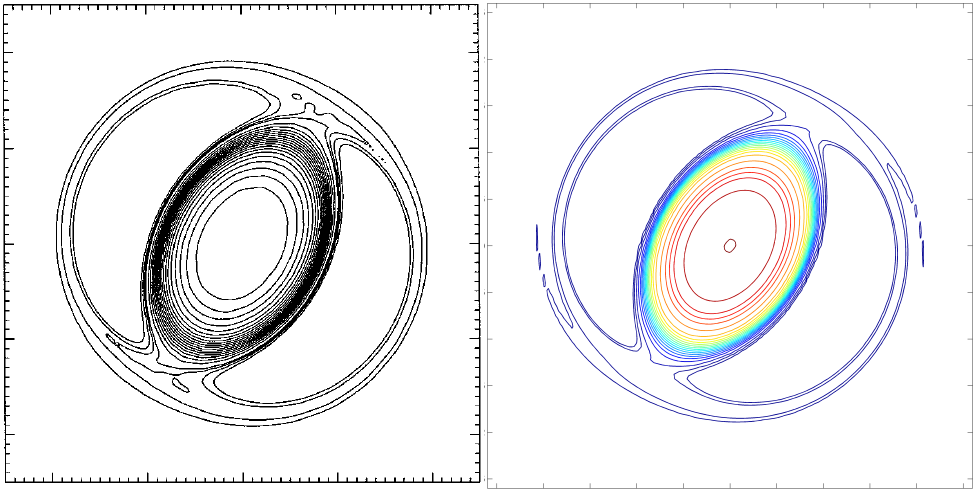
\includegraphics[width=0.8\textwidth]{KoumComp3.PNG}
\caption{\label{fig:KoumComp3}Comparison of vorticity, Koumoutsakos (left) and present method (right). From left to right: t=24; 23.98. Reprinted with permission from Elsevier.}
\end{figure}
}

\subsection{Comparison of Aspect Ratio(K)}
\frame{\frametitle{\subsecname}
\begin{figure}
\centering
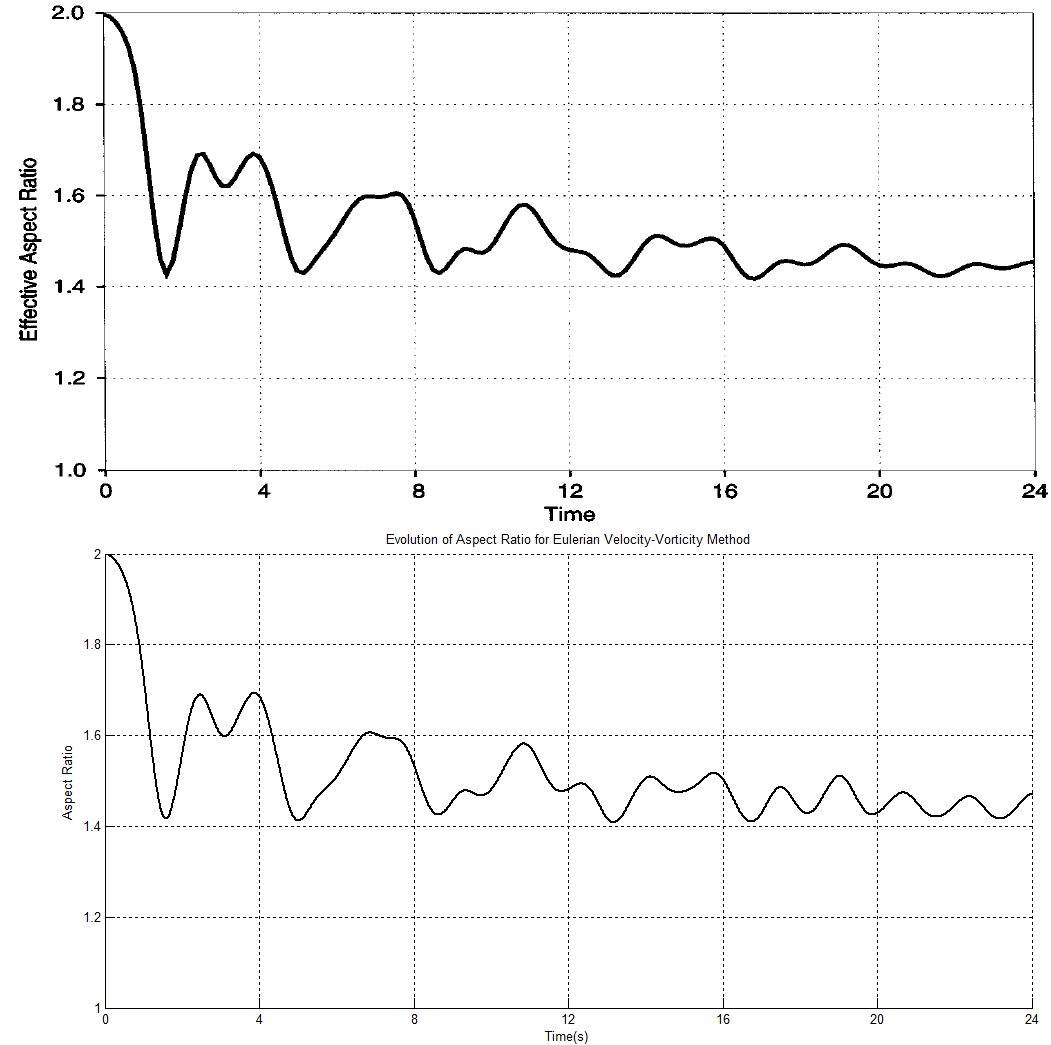
\includegraphics[width=0.65\textwidth]{AspectRatio.PNG}
\caption{\label{fig:AspectRatio}Comparison of effective aspect ratio, Koumoutsakos (top) and present method (bottom). Reprinted with permission from Elsevier.}
\end{figure}
}
\section{Discussion}
\subsection{Validation} 
\frame{\frametitle{\textbf{\secname}: \subsecname}
\begin{itemize}
\item Analytical: With proper choice of kernel, cutoff radius, stage-wise velocity evaluation, and matching velocity order method able to obtain solution within discretization error of exact solution for velocity and vorticity.
\item Qualitative: Excellent agreement in Strain test case even for test with far fewer DOFs
\item Good agreement in Koumoutsakos test case, with some minor deviation towards end of period studied and minor artifacting at vortex body boundaries.
\item DOFs required about equal to Koumoutsakos's results, despite being higher-order method.
\item Arm filaments and vortex body boundary challenging for polynomial basis functions, discontinuous derivatives affect bound on interpolation error.
\end{itemize}
}

\subsection{Convergence Rate} 
\frame{\frametitle{\subsecname}
\begin{itemize}
\item In Perlman test case, capable of near optimal convergence rates for stationary vortex test case.
\item Half-order less convergence rate for higher order methods due to lack of as many vorticity derivatives.
\item Non-optimal approximated convergence observed in Strain test case.
\item Choice of two options, cutoff radius too small and gradual decay of convergence to first order from optimal. Cutoff radius too large, constant but non-optimal order of convergence.
\item Tempting to blame smallest feature size or challenging evolution evolution for convergence, but testing with pairs of Perlman vortices shows same issues.
\end{itemize}
}

\subsection{Exact Biot-Savart Integration} 
\frame{\frametitle{\subsecname}
\begin{itemize}
\item Ideally: More accurately integrate B-S kernel, w/o extra error from de-singularization approximation.
\item Example: Calculate velocity component at particular point:
\be u_y(T_x) = \int \int \frac{\mathbf{x}-T_x}{2\pi r^2} \omega(\mathbf{x}) d\mathbf{x} \ee
\item $\omega$ is actually Lagrange interpolation of vorticity (with interp. values $z_{ij}$), so substitute:
\be u_y(T_x) = \frac{1}{2 \pi} \sum_i \sum_j z_{ij} \int \int \frac{x-T_x}{r^2} \; \ell_i(x) \ell_j(y) \;dx \;dy\ee
\item Note: Variable part of interp. occurs outside integral. We can pre-calculate integrals for all combinations and store.
\item Yields modified quadrature:
\be u(T_-)= \frac{1}{2 \pi} \sum_i \sum_j z_{ij} W_{(-, T_x,T_y,i,j)} \ee
\end{itemize}
}

\subsection{Exact B-S Integr.: Modified Kernel Values} 
\frame{\frametitle{\subsecname}
\begin{itemize}
\item How do these weights vary spatially wrt target point? Divide special weights by tensor product of standard Gauss-Legendre:
\be u_x= \frac{1}{2 \pi} \sum_i \sum_j z_{ij} \frac{W_{(i,j)}}{W_{GL}} W_{GL} \ee
\item Note: Can break into two parts; $\omega$ interpolation ($z_{ij}$) and B-S kernel values. Heuristically:
\be u_x= \frac{1}{2 \pi} \sum_i \sum_j z_{ij}  \overset{\sim}{k}_{ij} W_{GL} \ee
\item We have recovered something that looks like ``modified'' kernel values. How do they vary spatially?
\end{itemize}
}

\frame{\frametitle{\subsecname (cont.)}
\begin{itemize}
\item Modifications to standard kernel values are local; neighboring/adjacent elements. Promising for FMM acceleration.
\end{itemize}
\begin{figure}
\centering
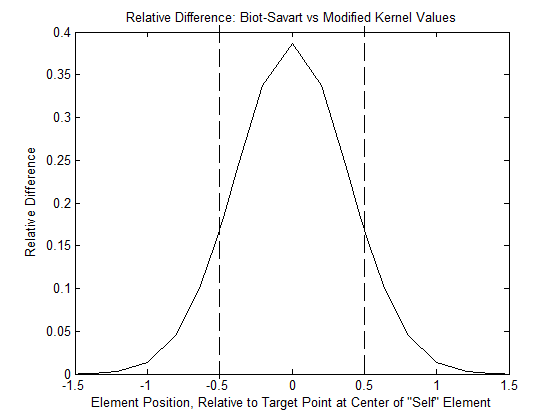
\includegraphics[width=.55\textwidth]{KernelModComp.PNG}
\caption{\label{fig:KernelModComp}Spatial variance of modified Biot-Savart kernels compared to that of tradition kernel values along a coordinate direction for a particular target point at the center of an element for a 6th order interpolation scheme}
\end{figure}
}

\section{Conclusion}
\frame[shrink]{\frametitle{\textbf{\secname}: \subsecname}
\begin{itemize}
\item Overarching goal of high-order solver capable of solving  inviscid incompressible vorticity-dominated flows in 2D met
\item Advective solver capable of mixed order flux handling was constructed capable of high-order convergence
\item High-order Biot-Savart evaluation routine using a direct summation approach created
\item Result is a complete high-order method for velocity-vorticity inviscid flow that integrates all necessary subsystems
\item Both solver and underlying Eulerian vortex approach were validated against analytical and qualitative test cases
\item $L^2$ error, vortex diagnostics, and convergence rate were measured
\item Method was shown capable of achieving near optimal convergence rate in some cases, ``high-order'' in others
\item Exact Biot-Savart integration points to promising potential for improved convergence and acceleration, additional validation needed.
\end{itemize}
}

\end{document}